\chapter{Potential Functions}
\label{chapter:potentialfunctions}

\FloatBarrier
\section{Introduction}

This section of the appendix covers the types of potential function and common choices of function used and details on how to use these in the potential fitting code.



\section{Functions}


%%%%%%%%%%%%%%%%%%%%%%%%%%%%%%%%%%%%%%%
% Ackland Embedding
%%%%%%%%%%%%%%%%%%%%%%%%%%%%%%%%%%%%%%%

\FloatBarrier
\subsection{Ackland Embedding}

\lstinputlisting[style=sFortran,caption={Ackland Embedding Fortran code}]{appendix/functions/pots_plots/fnc.ackland_embedding.f90}

\lstinputlisting[style=sOutputFile,caption={Ackland Embedding EAMPA input file}]{appendix/functions/pots_plots/ackland_embedding.pot}

\FloatBarrier
\begin{figure}[h]
  \begin{center}
    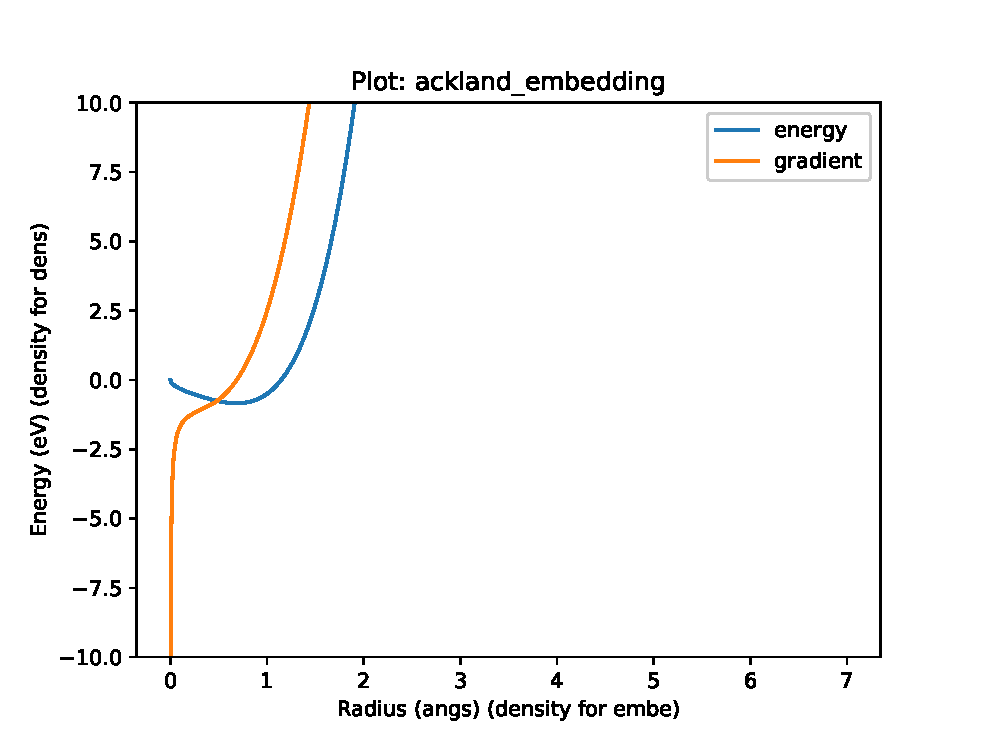
\includegraphics[width=0.7\linewidth]{appendix/functions/pots_plots/ackland_embedding.eps}
    \caption{Ackland Mendelev}
    \label{figure:functionsacklandmendelev}
  \end{center}
\end{figure}




%%%%%%%%%%%%%%%%%%%%%%%%%%%%%%%%%%%%%%%
% Buckingham
%%%%%%%%%%%%%%%%%%%%%%%%%%%%%%%%%%%%%%%

\FloatBarrier
\subsection{Buckingham}

\lstinputlisting[style=sFortran,caption={Buckingham Fortran code}]{appendix/functions/pots_plots/fnc.buckingham.f90}

\lstinputlisting[style=sOutputFile,caption={Buckingham EAMPA input file}]{appendix/functions/pots_plots/buckingham.pot}

\FloatBarrier
\begin{figure}[h]
  \begin{center}
    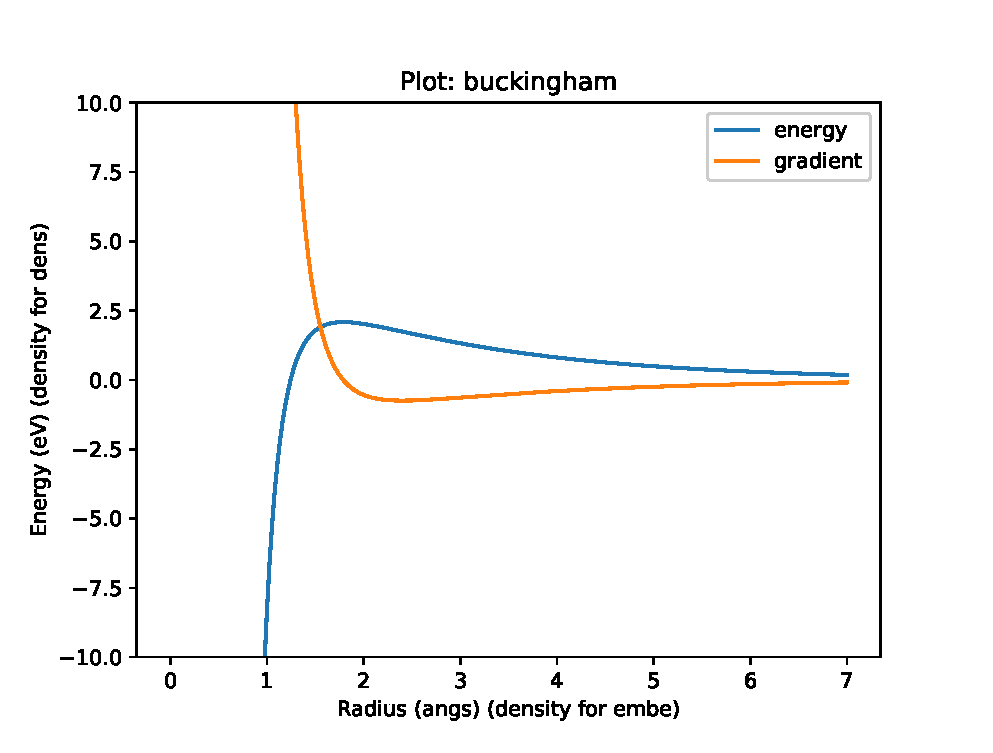
\includegraphics[width=0.7\linewidth]{appendix/functions/pots_plots/buckingham.eps}
    \caption{Buckingham}
    \label{figure:functionsbuckingham}
  \end{center}
\end{figure}




%%%%%%%%%%%%%%%%%%%%%%%%%%%%%%%%%%%%%%%
% Lennard Jones
%%%%%%%%%%%%%%%%%%%%%%%%%%%%%%%%%%%%%%%

\FloatBarrier
\subsection{Lennard Jones}

\lstinputlisting[style=sFortran,caption={Lennard Jones Fortran code}]{appendix/functions/pots_plots/fnc.lennard_jones.f90}

\lstinputlisting[style=sOutputFile,caption={Lennard Jones EAMPA input file}]{appendix/functions/pots_plots/lennard_jones.pot}

\FloatBarrier
\begin{figure}[h]
  \begin{center}
    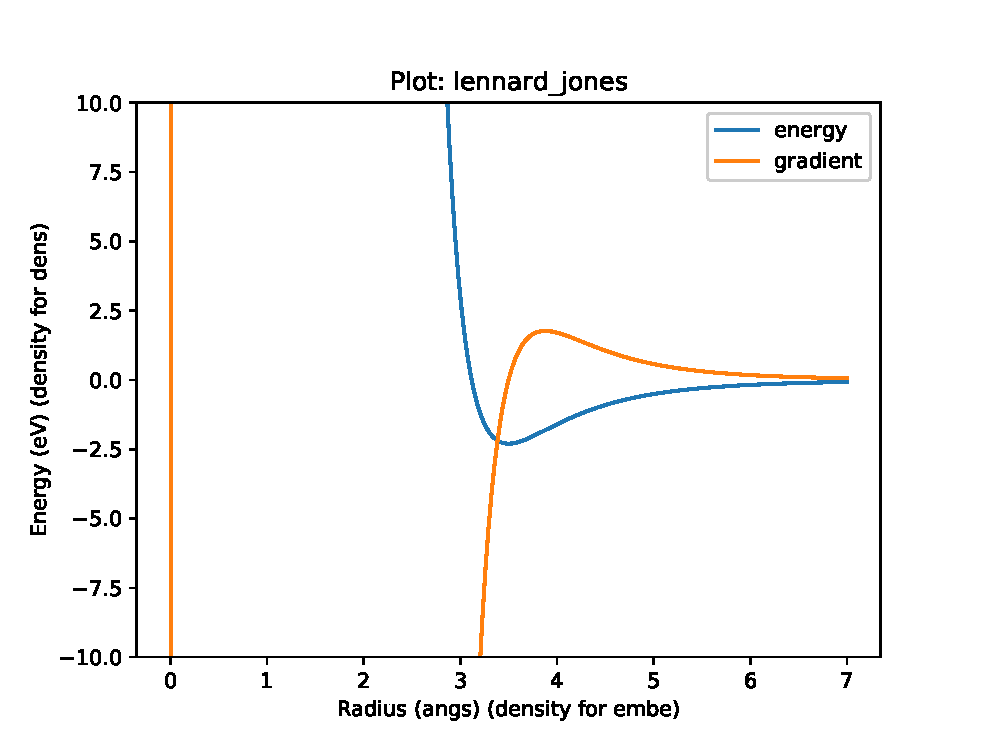
\includegraphics[width=0.7\linewidth]{appendix/functions/pots_plots/lennard_jones.eps}
    \caption{Lennard Jones}
    \label{figure:functionslennardjones}
  \end{center}
\end{figure}




%%%%%%%%%%%%%%%%%%%%%%%%%%%%%%%%%%%%%%%
% Mishin Density
%%%%%%%%%%%%%%%%%%%%%%%%%%%%%%%%%%%%%%%

\FloatBarrier
\subsection{Mishin Density}

\lstinputlisting[style=sFortran,caption={Mishin Density Fortran code}]{appendix/functions/pots_plots/fnc.mishin_density.f90}

\lstinputlisting[style=sOutputFile,caption={Mishin Density EAMPA input file}]{appendix/functions/pots_plots/mishin_density.pot}

\FloatBarrier
\begin{figure}[h]
  \begin{center}
    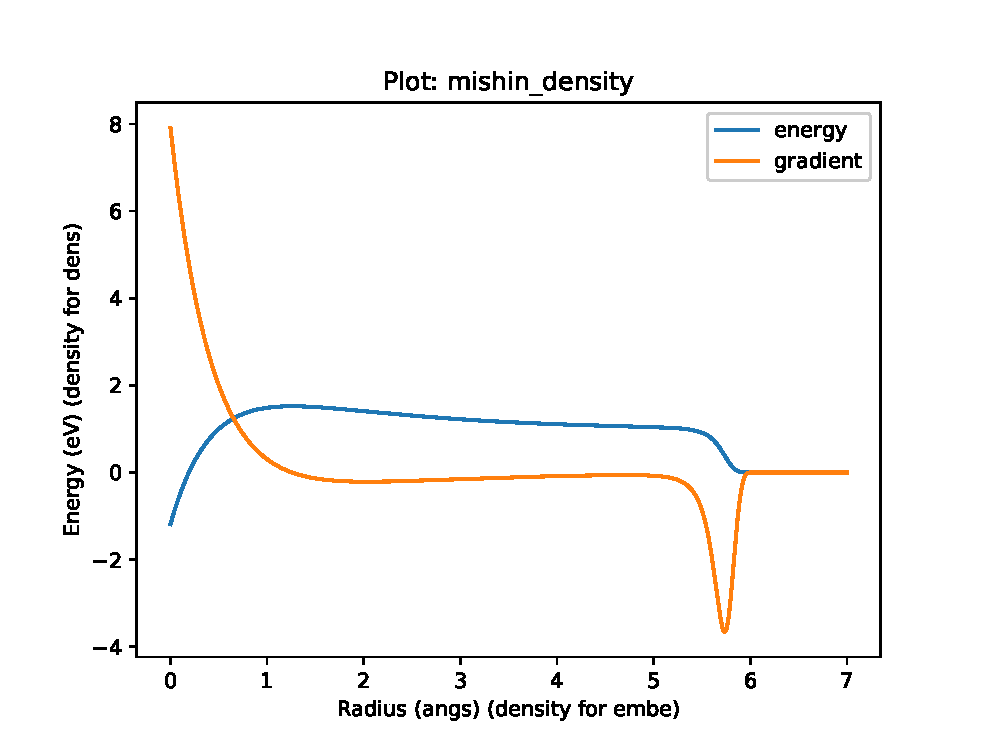
\includegraphics[width=0.7\linewidth]{appendix/functions/pots_plots/mishin_density.eps}
    \caption{Mishin Density}
    \label{figure:functionsmishindensity}
  \end{center}
\end{figure}




%%%%%%%%%%%%%%%%%%%%%%%%%%%%%%%%%%%%%%%
% Morse
%%%%%%%%%%%%%%%%%%%%%%%%%%%%%%%%%%%%%%%

\FloatBarrier
\subsection{Morse}

\lstinputlisting[style=sFortran,caption={Morse Fortran code}]{appendix/functions/pots_plots/fnc.morse.f90}

\lstinputlisting[style=sOutputFile,caption={Mishin Density EAMPA input file}]{appendix/functions/pots_plots/morse.pot}

\FloatBarrier
\begin{figure}[h]
  \begin{center}
    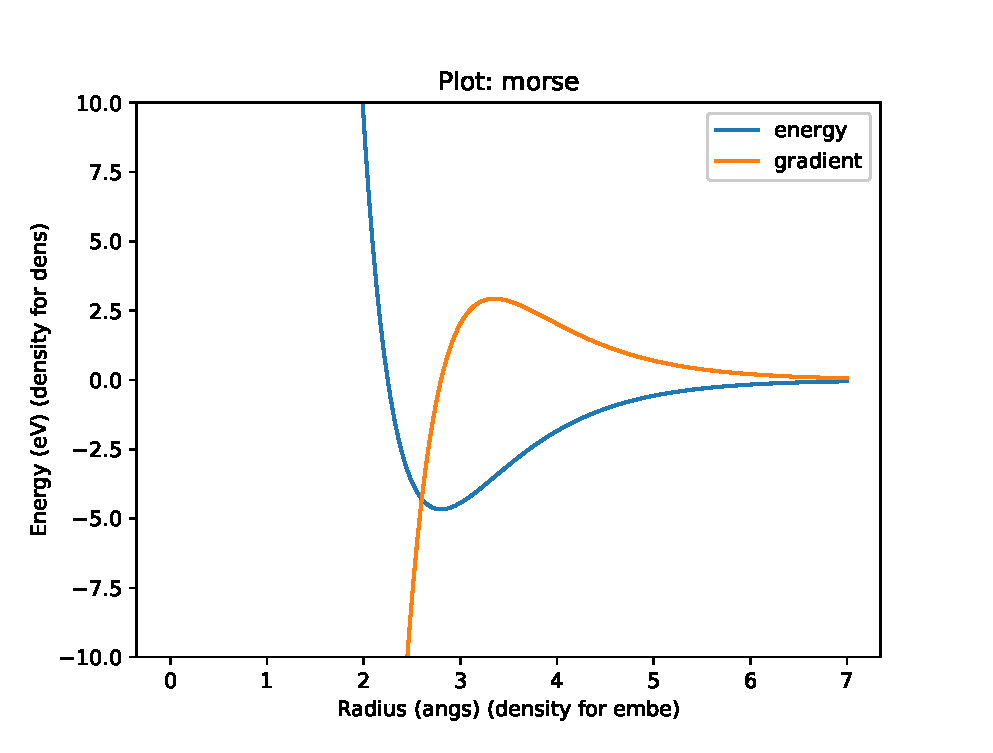
\includegraphics[width=0.7\linewidth]{appendix/functions/pots_plots/morse.eps}
    \caption{Morse}
    \label{figure:functionsmorse}
  \end{center}
\end{figure}




%%%%%%%%%%%%%%%%%%%%%%%%%%%%%%%%%%%%%%%
% Polynomial Embedding
%%%%%%%%%%%%%%%%%%%%%%%%%%%%%%%%%%%%%%%

\FloatBarrier
\subsection{Polynomial Embedding}

\lstinputlisting[style=sFortran,caption={Polynomial Embedding Fortran code}]{appendix/functions/pots_plots/fnc.polynomial_embedding.f90}

\lstinputlisting[style=sOutputFile,caption={Polynomial Embedding EAMPA input file}]{appendix/functions/pots_plots/polynomial_embedding.pot}

\FloatBarrier
\begin{figure}[h]
  \begin{center}
    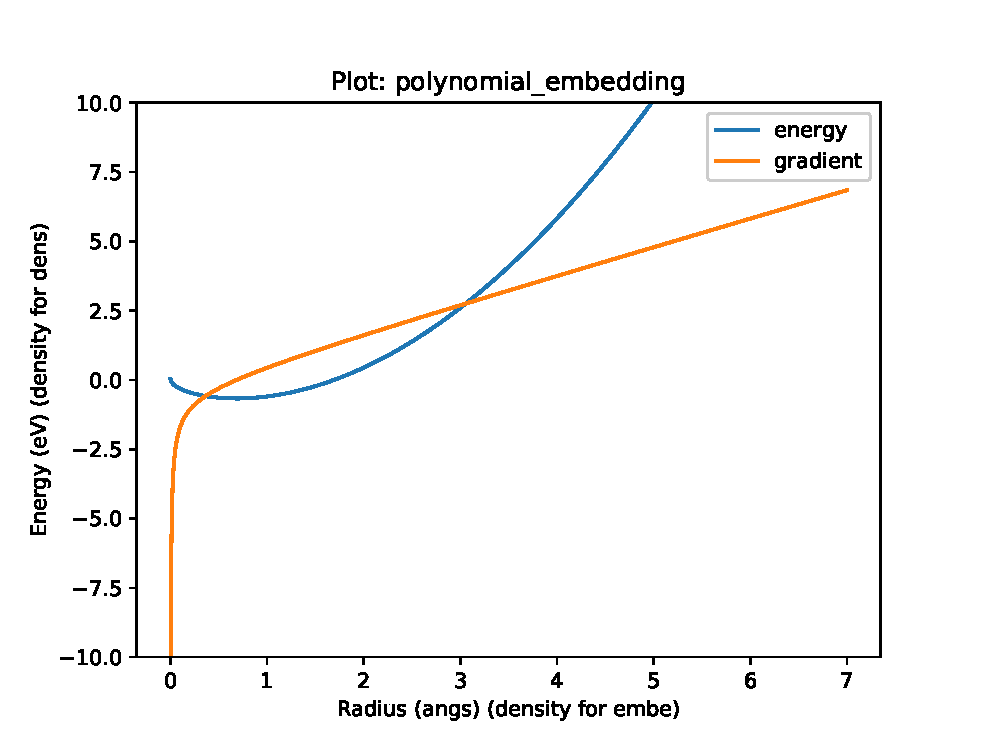
\includegraphics[width=0.7\linewidth]{appendix/functions/pots_plots/polynomial_embedding.eps}
    \caption{Polynomial Embedding}
    \label{figure:functionspolynomialembedding}
  \end{center}
\end{figure}




%%%%%%%%%%%%%%%%%%%%%%%%%%%%%%%%%%%%%%%
% Spline
%%%%%%%%%%%%%%%%%%%%%%%%%%%%%%%%%%%%%%%

\FloatBarrier
\subsection{Spline}

\lstinputlisting[style=sFortran,caption={Spline Fortran code}]{appendix/functions/pots_plots/fnc.spline.f90}

\lstinputlisting[style=sOutputFile,caption={Spline EAMPA input file}]{appendix/functions/pots_plots/spline.pot}

\FloatBarrier
\begin{figure}[h]
  \begin{center}
    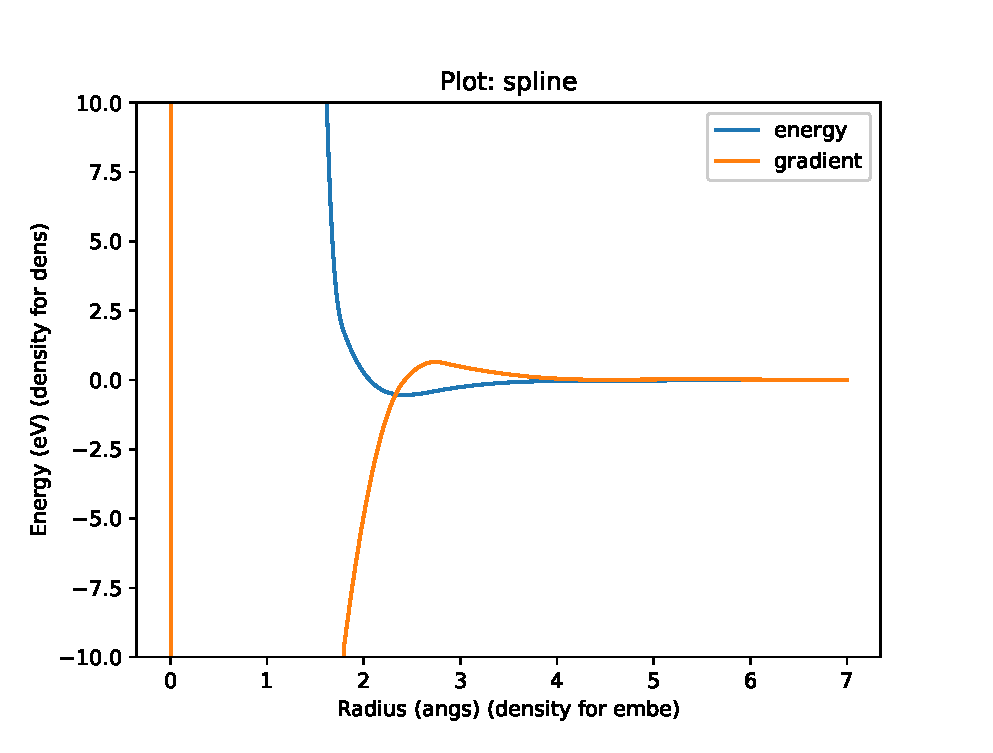
\includegraphics[width=0.7\linewidth]{appendix/functions/pots_plots/spline.eps}
    \caption{Spline}
    \label{figure:functionsspline}
  \end{center}
\end{figure}




%%%%%%%%%%%%%%%%%%%%%%%%%%%%%%%%%%%%%%%
% Slater 4s
%%%%%%%%%%%%%%%%%%%%%%%%%%%%%%%%%%%%%%%

\FloatBarrier
\subsection{Slater 4s}

\lstinputlisting[style=sFortran,caption={Slater 4s Fortran code}]{appendix/functions/pots_plots/fnc.slater_4s.f90}

\lstinputlisting[style=sOutputFile,caption={Slater 4s EAMPA input file}]{appendix/functions/pots_plots/slater_4s.pot}

\FloatBarrier
\begin{figure}[h]
  \begin{center}
    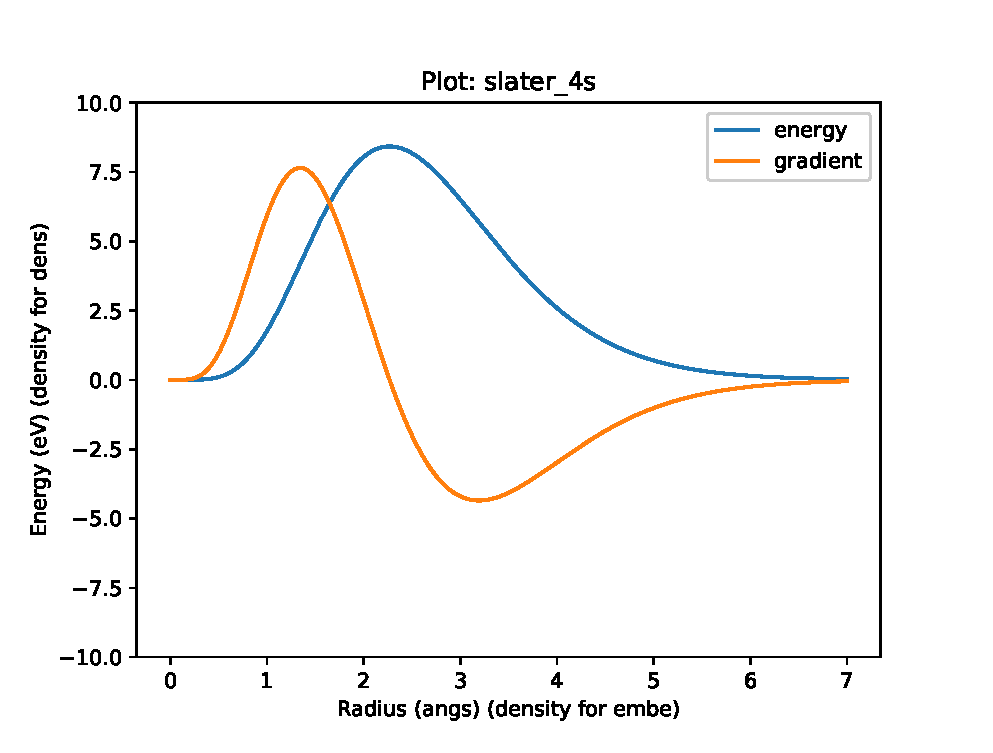
\includegraphics[width=0.7\linewidth]{appendix/functions/pots_plots/slater_4s.eps}
    \caption{Slater 4s}
    \label{figure:functionsslater4s}
  \end{center}
\end{figure}



%%%%%%%%%%%%%%%%%%%%%%%%%%%%%%%%%%%%%%%
% ZERO
%%%%%%%%%%%%%%%%%%%%%%%%%%%%%%%%%%%%%%%

\subsection{Zero}

\lstinputlisting[style=sFortran,caption={Zero Fortran code}]{appendix/functions/pots_plots/fnc.zero.f90}

\lstinputlisting[style=sOutputFile,caption={Zero EAMPA input file}]{appendix/functions/pots_plots/zero.pot}

\FloatBarrier
\begin{figure}[h]
  \begin{center}
    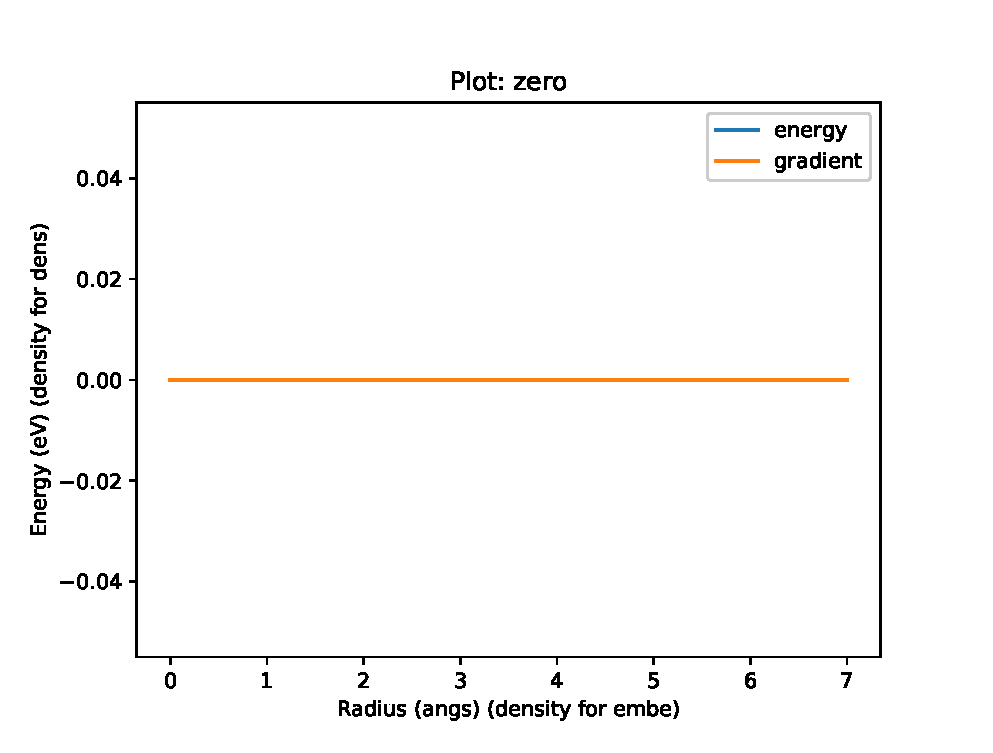
\includegraphics[width=0.7\linewidth]{appendix/functions/pots_plots/zero.eps}
    \caption{Zero}
    \label{figure:functionszero}
  \end{center}
\end{figure}


